\section{TAD}
\subsection{}
Um Tipo Abstrato de Dados, ou TAD, é um modelo matemático que define uma estrutura regular de dados e as funções que operam sobre essa estrutura. Geralmente, essa modelagem tem como propósito permitir uma representação computacional de um objeto de interesse. 

TADs permitem encapsulamento de código, legibilidade, coesão e um formalismo tão bom quanto necessário para se representar alguma estrutura de interesse. 

Caso uma função que opere sobre os dados precise ser modificada - mas mantenha o mesmo comportamento - não é necessário alterar todo o código. Apenas um aquele bloco de código precisa ser alterado. 

\subsection{}
Por definição, um cubo é um paralelepípedo cujas base, altura e profundidade são iguais. Dessa maneira, precisamos de um único elemento inteiro para representar o ``lado" do cubo. 

$$area\_cubo = \sum area \ faces = 6\cdot a^2$$

$$volume\_cubo = a^3$$

\begin{figure}[h!]
	\centering
	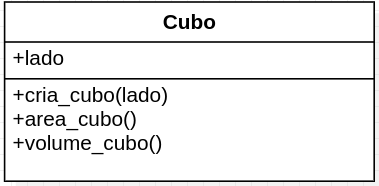
\includegraphics[width=4cm]{cubo_uml}
	\caption{TAD Cubo}
	\label{fig:cubouml}
\end{figure}

\lstinputlisting{../ex12/cubo.h}
\lstinputlisting{../ex12/cubo.c}
\lstinputlisting{../ex12/main.c}

Alguns testes a seguir: 

\begin{figure}[h!]
	\centering
	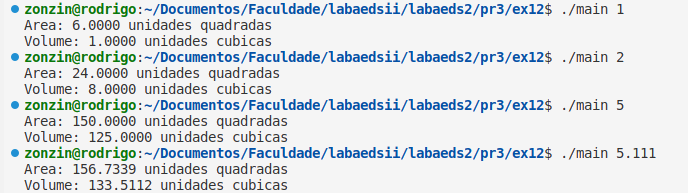
\includegraphics[height=3cm]{ex12_saida}
	\caption{Resultado}
	\label{fig:ex12saida}
\end{figure}

\newpage
\subsection{}
TAD para representar o conjunto de inteiros. Representado pelo tipo estruturado \textit{struct inteiros} onde existem os atributos:

	\textit{\textbf{int}* elementos}
	
	\textit{\textbf{int} n}

	\textit{\textbf{int} ocupado}\\


\textit{n} é um controlador de espaço para realocação de memória caso sejam inseridos mais elementos que o array \textit{elementos} comporta. 

De forma semelhante, \textit{ocupado} é um inteiro que representa a cardinalidade do conjunto.\\

Detalhes matemáticos e adaptações para implementação: 
 
\begin{itemize}
	\item Criar conjunto vazio:\\ 
		Existência da \textit{flag} $NaN= -9999$, pois $A = \{0, 0 , \ ...  \ , 0\} \neq \emptyset$. 
		
		No nosso caso, $\emptyset := \{-9999, -9999, \ ... \}$
		
	\item União de dois conjuntos. \\
	Dados dois Conjuntos $A$ e $B$, temos que $| A \cup B| = |A| + |B| - |A \cap B|$. 
	No nosso caso, $| A \cup B| := max(|A| \ , \ |B|)$ por facilidade de implementação. 
	
	\item Intersecção de dois conjuntos. 
	Dado dois conjuntos $A$ e $B$, $|A \cap B| = \{x : x \in A \ e \  x \in B\}$. A operação deve ser comutativa, logo $|A \cap B| = |B \cap A|$. 
	
	\item Diferença de dois conjuntos. \\
	Operação não comutativa. Dado dois conjuntos $A$ e $B$, temos que $A-B \neq B-A$. Prova: Seja $A = \{ 1, 2, 3, 4\}$ e $B = \{1, 3, 6, 9\}$. Temos $A-B = \{2, 4\}$ e $B-A = \{ 6, 9\}$. Obviamente, $A-B \neq B-A$. QED. Isso é respeitado. 
	
	\item Testar se dois conjuntos são iguais. \\
	Se dois conjuntos $A$ e  $B$ são iguais, então $A$ e $B$   têm mesma cardinalidade. Caso dois conjuntos não tenham o mesmo módulo, então podemos antecipar que são diferentes. 
	Caso tenham a mesma cardinalidade, precisamos ainda comparar elemento a elemento dos dois conjuntos. 
	
	\item  Testar se um conjunto é vazio. Duas abordagens: \textit{Lazy}: verificar se o número de elementos ocupados no conjunto é diferente de zero. Outra abordagem: verificar se os $|A|$ elementos em um conjunto $A$ é diferente da \textit{flag} -9999. 
\end{itemize}

\begin{figure}[h!]
	\centering
	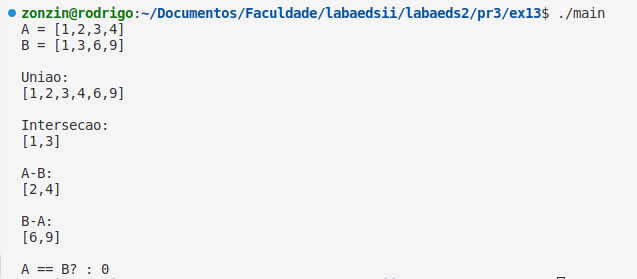
\includegraphics[width=0.7\linewidth]{ex13_saida}
	\caption{Resultado.}
	\label{fig:ex13saida}
\end{figure}


\lstinputlisting{../ex13/inteiros.h}
\lstinputlisting{../ex13/inteiros.c}
\lstinputlisting{../ex13/main.c}




